%!TEX root = ../report.tex
\chapter{Experiments}
\label{cha:experiments}
In order to thoroughly test our lexicon based classifier and our PMI lexicon, a series of experiments were conducted. Both to determine how well our classifier, utilizing the PMI lexicon, fared against other more complex classifiers, and to check the effect of using our classifier as a feature in a machine learning classifier. We also experimented with lexica of different sizes, and compared our system to the competing systems of SemEval 2016. Finally, we performed an ablation study to determine the most important features of both our lexicon creation process and our classification process.

\section{Transition from Graph to PMI}
\label{sec:transition_graph_pmi}
Through the initial phases of this thesis work, the graph propagation approach was our main and only lexicon creation approach. However, we encountered several problems with the graph approach: 
\begin{itemize}
    \item \textbf{Creating the seed set:} Since the value of all words in the lexicon are decided by their similarity to the words in the seed set, it is crucial to get the seed set right. A small seed often produced smaller lexica with weaker sentiment values since fewer words were propagating the values, while a large seed set often had problems with setting good starting sentiment values. For example, \textit{"good"}, \textit{"great"}, and \textit{"outstanding"} are all positive words, but their sentimental strength is different.
    \item \textbf{Creating the context vector:} The similarity between $n$-grams is calculated as similarity between their context vectors, described in Section~\ref{sec:context_vector}. While this approach may work for unigrams, the relationship between mutli-grams and their neighboring words is less clear.
    \item \textbf{Computational complexity of similarity measure:} Our implementation relied on calculating the cosine similarity for each word with every other word. This means that the overall computational complexity was exponential. In practice, we could not create any lexica with more than 8\thinspace000 elements.
    \item \textbf{Context similarity vs. Sentiment similarity:} Finally, context similarity is not always correlated with sentiment similarity. For example, the word \textit{"good"} and the word \textit{"bad"} are often used in similar contexts, \textit{"the weather is good/bad"}, \textit{"I'm good/bad at reading"}. 
\end{itemize}

After approximately two months of development without satisfactory results, we decided to try out the PMI approach identified through our research. After only a couple of days of development, the PMI approach outperformed our graph propagation approach, as shown in Table~\ref{tab:graph_vs_pmi}, which in turn led us to changing our main lexicon creation approach over to the PMI approach. Throughout the remainder of this chapter, only the lexica created through our PMI approach are tested in addition to the lexicon based classifier.

\begin{table}[t]
    \centering
    \begin{tabular}{|l|c|c|c|c|}
        \hline
        \textbf{System} & \textbf{2013} & \textbf{2014} & \textbf{2015} & \textbf{2016} \\ \hline
        Graph approach  & 0.4942 & 0.4844 & 0.4571 & 0.4744 \\ \hline
        PMI approach    & 0.6130 & 0.6170 & 0.5711 & 0.5685 \\ \hline
    \end{tabular}
    \caption[Early results of graph approach vs. PMI approach]{Early test results of graph approach vs. PMI approach tested on the 2013-2016 SemEval datasets.}
    \label{tab:graph_vs_pmi}   
\end{table}

\section{Grid Search}
\label{sec:grid_search}
For our system to perform as well as possible, we needed to find the optimal parameters. That included finding the optimal parameters for both our lexicon creator and our classifier, listed in Table~\ref{tab:lexicon_creator_parameters} and Table~\ref{tab:lexicon_classifier_parameters}. Because optimal classifier parameters depend on the particular lexicon being used, which again depends on the lexicon creator parameters, we needed to create our own grid search method for our thesis system. The method we ended up with was not a complete grid search where all combinations of parameter values are explored, but instead a simpler, iterative parameter search. The search consisted of a series of iterative steps, where we in each step tested all predefined values of a single parameter, while keeping all the other variables constant, in search of the value that provided the best result. When we were not able to improve the result by changing any of the parameter values, the search was done. Because we were not testing all possible combinations of values, the parameters found may be a local maximum, but the trade-off was necessary since testing each combination took 3 minutes on average.

\begin{table}[t]
    \setlength\tabcolsep{2pt}
    \begin{tabular}{| l | p{9cm} |}
        \hline
        \textbf{Parameter} & \textbf{Description} \\ \hline
        maxNGramLength & Longest $n$-gram to include in vocabulary \\ \hline
        minNGramFreq & Minimum $n$-gram occurrence frequency to include in vocabulary \\ \hline
        minNGramPMI & Minimum $n$-gram PMI value to include in vocabulary \\ \hline
        minOccurrence & Minimum $n$-gram occurrence in polarized dataset to include in lexicon \\ \hline
        minSentiment & Minimum $n$-gram absolute sentiment value to include in lexicon \\ \hline
    \end{tabular}
    \caption{List of lexicon creator parameters}
    \label{tab:lexicon_creator_parameters}
\end{table}

\begin{table}[t]
    \setlength\tabcolsep{2pt}
    \begin{tabular}{| l | p{9cm} |}
        \hline
        \textbf{Parameter} & \textbf{Description} \\ \hline
        negationValue & The negation constant $N$ in Equation~\ref{eq:token_sentiment} \\ \hline
        exclamationIntensifier & Intensification constant for tokens inside sentence ending with an exclamation mark \\ \hline
        questionIntensifier & Intensification constant for tokens inside sentence ending with a question mark \\ \hline
        negationLength & Number of tokens after a negation cue that are considered negated \\ \hline
        classThreshLower & Threshold between the \textit{negative} and the \textit{neutral} sentiment classification \\ \hline
        classThreshHigher & Threshold between the \textit{neutral} and the \textit{positive} sentiment classification \\ \hline
    \end{tabular}
    \caption{List of lexicon classifier parameters}
    \label{tab:lexicon_classifier_parameters}
\end{table}

\section{Quality of SemEval Datasets}
\label{sec:criticism_semeval}
Through system tests performed during development, the SemEval 2016 results and the final system tests described in the following section, our scepticism towards the overall quality of the SemEval datasets of 2015 and 2016 in particular, was sparked. As discovered in the following section as well as through the SemEval 2016 results, the performance of all the classifiers drops drastically from the tests on the 2013 dataset to the 2016 dataset. This in turn led us to perform a few experiments on the datasets to see if we could back up our suspicions of a lower quality of the 2015 and 2016 SemEval datasets. We started our experiments by finding the number of duplicate tweets in the four datasets. For the datasets with duplicate tweets we checked whether or not the duplicate tweets were given the same classification label and counted the number of duplicates with different labels. \\

\begin{table}[t]
    \centering
    \begin{tabular}{|l|c|c|}
        \hline
        \textbf{Dataset} & \textbf{Duplicates} & \textbf{Different Classification}\\ \hline
        2013-test & 1.62 & 0.32 \\ \hline
        2014-test & 0.00 & 0.00 \\ \hline
        2015-test & 6.94 & 2.09 \\ \hline
        2016-test & 3.88 & 1.36 \\ \hline
    \end{tabular}
    \caption[SemEval dataset experiments]{SemEval dataset experiments, all values are per thousand tweets}
    \label{tab:dataset_experiments}   
\end{table}

As we can see from Table~\ref{tab:dataset_experiments} there are only 1.62 duplicated tweets per thousand tweets in the 2013 dataset and none in the 2014 dataset. In addition only 0.32 tweets per thousand found in the 2013 dataset had different classification label. For the two other datasets on other hand, we found significantly more duplicates that were classified differently. However, the amount of duplicated tweets with different classification is in comparison to the dataset size relatively small, and will on its own not impact the results noticeably. More importantly the numbers point to a possible preference difference among the used annotators, when it comes to what they assume is a polarized tweet (positive or negative) and what is a neutral tweet. The method of collecting and annotating tweets, described by \cite{SemEval:2016:task4}, has stayed the same since 2013, where Amazons Mechanical Turk\footnote{A tool that enables outsourcing of tasks to Internet workers. Given a task and a selling price, Internet workers perform the task and are subsequently paid for it.} is used for annotating. Among the duplicate tweets identified, there were no tweets classified as both negative and positive. 


\section{System Performance}
\label{sec:system_performance}
To test the overall performance of our system, five main experiments were conducted: a system comparison experiment, a system feature experiment, lexicon comparison experiment, lexicon classifier in SemEval 2016 experiment and lexicon size comparison experiment.  

\subsection{System Comparison}
\label{sec:system_comparison}
The system comparison experiment consisted of a series of tests where our lexicon based classifier, utilizing our PMI lexicon, was compared against other previously developed NTNU systems along with our Initial Experiment system (see Section~\ref{ch:initial_experiment}) and a lexicon based system \textit{VADER Sentiment}, introduced in Section~\ref{sec:vaderSentiment}. The comparison was done based on the systems' test results across four different datasets as shown in Table~\ref{tab:master_system_comparison}. \\

\begin{table}[t]
    \centering
    \begin{tabular}{l|l|c|c|c|c|}
        \cline{2-6}
        & \textbf{System} & \textbf{Precision} & \textbf{Recall} & \textbf{F1-Score} & \textbf{Time} \\
        \cline{1-6}
        \multirow{5}{*}{\rot{2013}} & \citeauthor{SelmerBrevik} & 0.6787 & 0.6644 & 0.6482 & 0.36 \\
        \cline{2-6}
        & \citeauthor{FaretReitan}      & 0.731  & 0.697  & 0.688  & \textasciitilde{}180  \\
        \cline{2-6}
        & VADER Sentiment               & 0.6540 & 0.6573 & 0.6508 & 1.29 \\
        \cline{2-6}
        & Initial Experiment            & 0.7209 & 0.7120 & 0.7073 & 74.01 \\
        \cline{2-6}
        & \textbf{Lexicon Classifier}   & 0.6866 & 0.6803 & 0.6748 & 0.04 \\
        \hhline{======|}
        
        \multirow{5}{*}{\rot{2014}} & \citeauthor{SelmerBrevik} & 0.7071 & 0.6667 & 0.6614 & 0.17 \\
        \cline{2-6}
        & \citeauthor{FaretReitan}      & 0.738  & 0.684  & 0.684  & \textasciitilde{}93  \\
        \cline{2-6}
        & VADER Sentiment               & 0.6536 & 0.6421 & 0.6441 & 0.63 \\
        \cline{2-6}
        & Initial Experiment            & 0.7091 & 0.6832 & 0.6847 & 41.38 \\
        \cline{2-6}
        & \textbf{Lexicon Classifier}   & 0.6818 & 0.6554 & 0.6578 & 0.02 \\
        \hhline{======|}
        
        \multirow{4}{*}{\rot{2015}} & \citeauthor{SelmerBrevik} & 0.6615 & 0.6305 & 0.6155 & 0.26 \\
        \cline{2-6}
        & VADER Sentiment               & 0.6310 & 0.6201 & 0.6197 & 0.99 \\
        \cline{2-6}
        & Initial Experiment            & 0.6862 & 0.6548 & 0.6527 & 64.80 \\
        \cline{2-6}
        & \textbf{Lexicon Classifier}   & 0.6483 & 0.6213 & 0.6201 & 0.03 \\
        \hhline{======|}
        
        \multirow{4}{*}{\rot{2016}} & \citeauthor{SelmerBrevik} & 0.6101 & 0.6184 & 0.6093 & 2.39 \\
        \cline{2-6}
        & VADER Sentiment               & 0.5939 & 0.5919 & 0.5928 & 8.63 \\
        \cline{2-6}
        & Initial Experiment            & 0.6461 & 0.6434 & 0.6431 & 538.88 \\
        \cline{2-6}
        & \textbf{Lexicon Classifier}   & 0.6085 & 0.6028 & 0.6032 & 0.19 \\
        \hhline{======|}
    \end{tabular}
    \caption[Sentiment classifier performance results]{Performance results of Sentiment classifiers tested on the 2013-2016 SemEval datasets.}
    \label{tab:master_system_comparison}   
\end{table}

All systems except our lexicon classifier utilize a \ac{svm} in the classification process. Although the \textit{VADER Sentiment} is a lexicon based system, and the most similar system to our lexicon based classifier, its output include several numerical values and not a sentiment class, therefore an additional classification step using \ac{svm} is required. \\

On the 2013 dataset our lexicon classifier is only beaten, regarding precision, recall and F1-score, by our Initial Experiment system and the system by \citeauthor{FaretReitan}, which by far are the most sophisticated systems of the five compared systems. More importantly our lexicon classifier beats both the system of \citeauthor{SelmerBrevik} and the \textit{VADER Sentiment} system, both of which also use machine learning approaches, against our simple lexicon approach. On the 2014 and 2016 datasets our lexicon classifier is also narrowly beaten by \citeauthor{SelmerBrevik}, while on the 2015 dataset our classifier achieves a higher F1-score. The \textit{VADER Sentiment} system scores below our classifier across all performance measures on all of the four datasets. \\

In addition to our system achieving scores relatively close to the more sophisticated machine learning based systems, our system significantly outperforms all of the other systems when it comes to the run-time. Even on the smallest dataset, our system executes approximately $8.5$ times faster than the second fastest system and approximately 2\thinspace000 times faster than our Initial Experiment, being the slowest. With an execution time of 0.19 seconds on the 2016 dataset, our classifier classifies tweets with a speed of 108\thinspace600 tweets per second, against the speed of our Initial Experiment system with $38$ tweets per second. \\

As mentioned in Section~\ref{sec:criticism_semeval} the performance across all compared systems drops significantly from the 2013 and 2014 datasets to the 2015 and 2016 datasets. Although one can argue that the results might be an effect of using a training dataset from 2013 to train the classification model of the \ac{svm} systems or using the \textit{AFINN} lexicon by \cite{AFINN} to create the \textit{Labeled} dataset for our lexicon creator, much points in the direction of a degradation of quality of the SemEval datasets.


\subsection{Classifier as a Feature}
From the ablation study conducted in our Initial Experiment, described in Section~\ref{sec:test_results}, we found that the sentiment lexica feature and the \textit{VADER Sentiment} feature, which also is a lexicon based feature, were the two single most important features of the system. Based on that knowledge we wanted to see whether or not our lexicon based classifier, used as a feature in our Initial Experiment system, could improve the system performance further. Therefore, we first ran our Initial Experiment system on the same four datasets as earlier, before running the same tests on the system with our lexicon based classifier as a feature. \\

\begin{table}[t]
    \centering
    \begin{tabular}{|l|c|c|c|c|}
        \hline
        \textbf{System} & \textbf{2013} & \textbf{2014} & \textbf{2015} & \textbf{2016} \\ \hline
        Initial Experiment & 0.7073 & 0.6847 & 0.6527 & 0.6431 \\ \hline
        Initial Experiment + Lexicon Classifier & 0.7216 & 0.6911 & 0.6586 & 0.6356 \\ \hline
    \end{tabular}
    \caption[Results of Initial Experiment with PMI lexicon]{Results of Initial Experiment with PMI lexicon tested on 2013-2016 SemEval datasets.}
    \label{tab:initial_experiment_with_lexicon}   
\end{table}

From Table~\ref{tab:initial_experiment_with_lexicon} we can see a clear increase in performance in terms of F1 score, increasing the F1 score from $0.7073$ to $0.7216$ on the 2013 dataset when adding our lexicon based classifier as a feature. There is also an increase in F1 score on the 2014 and 2015 datasets, although not as apparent. On the 2016 dataset on the other hand, the performance in terms of F1 actually drops below the F1 score of our Initial Experiment system. As far as we can tell, there is no obvious reason for this drop in performance on the 2016 dataset.


\subsection{Lexicon Comparison}
\label{sec:lexicon_comparison}
Because a large part of our thesis revolves around the creation of a sentiment lexicon, we found it relevant to compare our PMI lexicon against other previously created sentiment lexica. Since the sentiment lexicon \textit{Sentiment140} was also created using a PMI approach, it became an obvious choice for comparison in addition the \textit{AFINN} lexicon used in the creation of our \textit{Labeled} dataset. The comparison was done by running our lexicon based classifier on the four SemEval datasets as done in the previous tests, using the \textit{Sentiment140}, \textit{AFINN} and our PMI lexicon as lexicon, respectively. \\

\begin{table}[t]
    \centering
    \begin{tabular}{|l|c|c|c|c|}
        \hline
        \textbf{Lexicon} & \textbf{2013} & \textbf{2014} & \textbf{2015} & \textbf{2016} \\ \hline
        Sentiment140            & 0.5260 & 0.5415 & 0.4788 & 0.5186 \\ \hline
        AFINN                   & 0.6259 & 0.6009 & 0.5801 & 0.5882 \\ \hline
        \textbf{PMI Lexicon}    & 0.6748 & 0.6578 & 0.6201 & 0.6032 \\ \hline
    \end{tabular}
    \caption[Performance comparison of different lexica with our classifier]{Performance comparison of different lexica with our classifier after being tested on the 2013-2016 SemEval datasets.}
    \label{tab:lexicon_comparison}   
\end{table}


As we can see from Table~\ref{tab:lexicon_comparison} our PMI lexicon outperforms the other two sentiment lexica, in terms of F1 score. \textit{AFINN} is the closest, with the smallest difference of approximately $0.015$ on the 2016 dataset. Even though the difference between \textit{AFINN} and our PMI lexicon is quite significant, the difference is even greater between \textit{Sentiment140} and our PMI lexicon with the smallest difference of approximately $0.085$ on the 2016 dataset. \\

Although the results seem to point to the conclusion that our lexicon is the best of the three, there are multiple reasons why this might not be the case. During development of our lexicon creator and our lexicon based classifier, we always focused on the fact that they were going to be used together. The PMI lexicon was therefore specifically tailored to work well with our classifier. Negators and intensifiers were for example left out of our lexicon because we knew we were going to handle negation and intensification in our classifier, and both the lexicon creator and the classifier utilizes the same preprocessing method. \\

For the \textit{AFINN} lexicon, we believe the results are not heavily affected by our specialized classifier. The \textit{AFINN} lexicon only contains words without special characters and has a single sentiment value per lexicon entry similarly to our PMI lexicon. By looking at the contents of the \textit{Sentiment140} lexicon on the other hand, it becomes apparent that we were not able to utilize all of the features the lexicon provides with our classifier. The two main reasons for this are the use of a different preprocessing method and having two values per lexicon entry, one for non-negated context and one for negated context. Since our preprocessing method removes all non-alphanumerical characters except for characters forming an emoticon, there are many entries in the \textit{Sentiment140} lexicon our classifier would never be able to use. In addition, all of the negated context values in \textit{Sentiment140} would also never be used by our classifier because of negation being handled differently. We therefore believe that given the combination of the aforementioned features our classifier were unable to utilize, no accurate conclusion can be drawn based on the results in Table~\ref{tab:lexicon_comparison} for the \textit{Sentiment140} lexicon. We do, however, believe that our method of creating a labeled dataset for the lexicon creator is slightly better than the hashtag and emoticon approach used in the creation of the \textit{Sentiment140} lexicon, and that the use of $n$-grams larger than just unigrams and bigrams benefits our lexicon. \\

\begin{figure}[t]
    \centering
    \begin{subfigure}[b]{0.49\textwidth}
        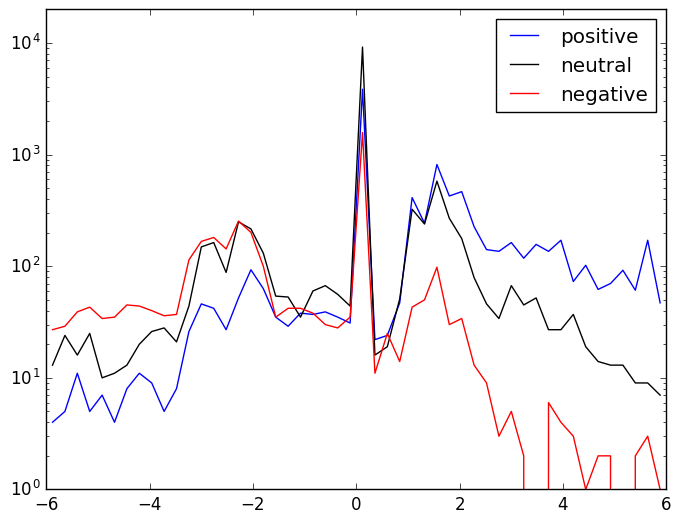
\includegraphics[width=\textwidth]{./figs/distrib/pmi}
        \caption{Histogram for PMI lexicon}
        \label{fig:distrib_pmi}
    \end{subfigure}
    \begin{subfigure}[b]{0.49\textwidth}
        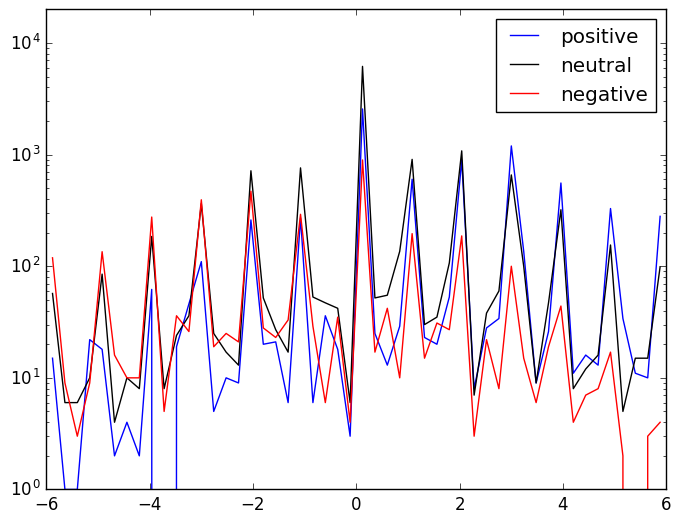
\includegraphics[width=\textwidth]{./figs/distrib/afinn}
        \caption{AFINN lexicon}
        \label{fig:distrib_afinn}
    \end{subfigure}
    \caption{Sentiment value histogram of PMI vs. AFINN Lexicon}
    \label{fig:distrib_comparison}
\end{figure}

Because the comparison of our PMI lexicon and the \textit{AFINN} lexicon is the most reasonable comparison among the three lexica in Table~\ref{tab:lexicon_comparison} a figure visualizing the differences has been created. In Figure~\ref{fig:distrib_comparison} two graphs depicting the distribution of positive, negative and neutral tweets given their sentiment values predicted by our classifier, are shown. In Figure~\ref{fig:distrib_pmi} we can see a clear distinction between the classes. For negative sentiment values, most tweets were negative, second most neutral and least positive. On the other hand, for positive sentiment values, most tweets were positive, second most neutral and least negative. For sentiment values close to zero, neutral tweets are the most common. In Figure~\ref{fig:distrib_afinn}, showing the distribution for the \textit{AFINN} lexicon, we can immediately identify a clear difference from the distribution graph of our PMI lexicon. Where the classes are distinctly separated in the distribution graph for our PMI lexicon, the classes are much closer and overlapping in the distribution graph for the \textit{AFINN} lexicon. One can for the most part identify the same order of classes on both the negative and the positive side, but the distance between them is generally much closer in the distribution graph for the \textit{AFINN} lexicon. The zig-zagged pattern in Figure~\ref{fig:distrib_afinn} is due to \textit{AFINN} lexicon only using integer sentiment values. The separability of the different classes displayed in the graphs shows why our PMI lexicon will generally classify more positive, negative and neutral tweets correctly.


\subsection{Lexicon Classifier in SemEval 2016}
After participating in SemEval 2016 with our Initial Experiment system, we wanted to explore how our lexicon based classifier would affect the final result used as a feature, as well as how it would perform on its own compared to the other participants. \\

\begin{table}[H]
    \centering
    \resizebox{\textwidth}{!}{
    \begin{tabular}{|l|ll|lll|l|l|l|}
    \hline
   & \multicolumn{7}{c|}{\bf F1-Score} & \textbf{Accur.} \\ \cline{2-9}
   & \multicolumn{2}{c|}{\bf 2013} & \multicolumn{3}{c|}{\bf 2014} & \multicolumn{1}{c|}{\bf 2015} & \multicolumn{1}{c|}{\bf 2016} & \multicolumn{1}{c|}{\bf 2016} \\
   \multicolumn{1}{|c|}{\bf System} & \bf Tweet & \bf SMS & \bf Tweet & \bf Tweet & \bf Live- & \bf Tweet & \bf Tweet & \bf Tweet \\
   &  &  & \bf & \bf sarca. & \bf Jour. & & & \\
\hline
NTNUSentEval & 0.623$_{11}$ & 0.641$_{1}$ & 0.651$_{10}$ & 0.427$_{13}$ & 0.719$_{3}$ & 0.599$_{13}$ & \bf 0.583$_{11}$ & 0.643$_{2}$ \\
w/ Lexicon Classifier & 0.648$_{9}$ & 0.659$_{1}$ & 0.667$_{8}$ & 0.438$_{12}$ & 0.707$_{3}$ & 0.609$_{11}$ & \bf 0.583$_{11}$ & 0.636$_{4}$ \\
Lexicon Classifier & 0.597$_{17}$ & 0.565$_{14}$ & 0.614$_{18}$ & 0.284$_{34}$ & 0.590$_{21}$ & 0.554$_{20}$ & \bf 0.541$_{19}$ & 0.603$_{9}$ \\
    \hline
    \end{tabular}}
    \caption[Alternative SemEval 2016 results]{Alternative F1-scores and accuracy results for SemEval 2016 if we had submitted different systems instead. Ordered by F1-scores on the 2016 dataset.}
    \label{tab:alternative_semeval_results}
\end{table}

As shown in Table~\ref{tab:alternative_semeval_results}, using our lexicon based classifier as a feature in our Initial Experiment system \textit{NTNUSentEval}, the F1-score on the 2016 dataset is the same as the score of \textit{NTNUSentEval}. However, on all other datasets except for the Live-Journal dataset, the F1 score is increased, and our placement improved. The performance of our lexicon based classifier on its own is significantly lower, but would still have ended up on 19th place out of the competing 34 systems. 

\subsection{Lexicon Size Comparison}
\label{sec:lexicon_size_comparison}
Another interesting aspect we wanted to explore was how the size of the created sentiment lexicon affected the performance. In order to explore that, eight sentiment lexica of sizes ranging from 500 to 200\thinspace000 entries were created and tested on the four SemEval datasets. \\

\begin{table}[t]
    \centering
    \begin{tabular}{|r|c|c|c|c|}
        \hline
        \textbf{Lexicon Size} & \textbf{2013} & \textbf{2014} & \textbf{2015} & \textbf{2016} \\ \hline
            500                     & 0.3387 & 0.2736 & 0.3029 & 0.3936 \\ \hline
          1\thinspace500            & 0.6533 & 0.6343 & 0.6049 & 0.6016 \\ \hline
      \bf 3\thinspace000            & 0.6748 & 0.6578 & 0.6201 & 0.6032 \\ \hline
         10\thinspace000            & 0.6674 & 0.6507 & 0.6201 & 0.6038 \\ \hline
         25\thinspace000            & 0.6328 & 0.6203 & 0.6020 & 0.6011 \\ \hline
         50\thinspace000            & 0.6052 & 0.6092 & 0.5650 & 0.5976 \\ \hline
        100\thinspace000            & 0.6040 & 0.6090 & 0.5648 & 0.5851 \\ \hline
        200\thinspace000            & 0.5965 & 0.6020 & 0.5626 & 0.5938 \\ \hline
    \end{tabular}
    \caption[Comparison of different sized PMI lexica]{Comparison of different sized PMI lexica after being tested on the 2013-2016 SemEval datasets.}
    \label{tab:comparison_different_size_lexica}   
\end{table}

As we can see from Table~\ref{tab:comparison_different_size_lexica}, as long as the lexicon size is above a certain threshold, the overall performance remain acceptable. We do, however, see a continuous drop in performance when the lexicon size passes 10\thinspace000 entries. \\

The best performing lexicon from the above test, has 3\thinspace000 entries, which is quite interesting looking at the \textit{Sentiment140} lexicon with approximately 300\thinspace000 entries in comparison. More words and phrases do not necessary lead to better results. Although that statement is valid for our lexicon creation approach, no general conclusion can be drawn. Our lexicon creation process as described in Section~\ref{sec:pmi_lexicon_creation}, only includes vocabulary entries also found in the \textit{Labeled} dataset containing $6.25$ million labeled tweets. Although the size of the \textit{Labeled} dataset is large enough, and its contents are mostly classified correctly, many relevant words and phrases might not have been included. Since the \textit{Labeled} dataset is created, as described in Section~\ref{sec:labeled}, using the \textit{AFINN} lexicon and an inclusion threshold of absolute sentiment value, both tweets with few positive and negative words, and positive and negative tweets with only a few words found in \textit{AFINN} are left out. A better method of creating a labeled dataset might therefore be the solution to create larger lexica with better performance. \\

In addition to the F1-score of the different sized lexica, we also wanted to see the difference in coverage between them. In terms of coverage, four different measures were used: 
\begin{itemize}
    \item \textbf{NZS} (Tweets with Non-Zero Sentiment): Ratio of tweets where final predicted sentiment value was $\neq 0$.
    \item \textbf{TwM} (Tweets with Multi-grams): Ratio of tweets that included at least one multi-gram from the lexicon.
    \item \textbf{WiL} (Words in Lexicon): Ratio of words in tweets found in the lexicon.
    \item \textbf{FWiL} (Frequent Words in Lexicon): Ratio of top 1\thinspace000 most common, non-stop-word words found in the lexicon.
\end{itemize}  

\begin{table}[t]
    \centering
    \begin{tabular}{|r|c|c|c|c|}
        \hline
        \textbf{Lexicon Size} & \textbf{NZS} & \textbf{TwM} & \textbf{WiL} & \textbf{FWiL} \\ \hline
            500                     & 0.0435 & 0.0066 & 0.3567 & 0.0081 \\ \hline
          1\thinspace500            & 0.3902 & 0.0086 & 0.3793 & 0.0655 \\ \hline
      \bf 3\thinspace000            & 0.4726 & 0.0412 & 0.3632 & 0.0826 \\ \hline
         10\thinspace000            & 0.4922 & 0.0702 & 0.3647 & 0.0846 \\ \hline
         25\thinspace000            & 0.8421 & 0.1788 & 0.4012 & 0.1712 \\ \hline
         50\thinspace000            & 0.9968 & 0.3322 & 0.5229 & 0.4371 \\ \hline
        100\thinspace000            & 0.9992 & 0.4703 & 0.6122 & 0.7019 \\ \hline
        200\thinspace000            & 0.9996 & 0.6012 & 0.6692 & 0.9889 \\ \hline
    \end{tabular}
    \caption{Lexicon coverage overview}
    \label{tab:lexicon_coverage}   
\end{table}

From Table~\ref{tab:lexicon_coverage} the results of our coverage experiment are shown. Interestingly the best performing lexicon with a size of 3\thinspace000 only contains words found in $47\%$ of the tweets. That means, that almost half of the tweets end up with a sentiment score of zero and are classified as neutral. In addition only approximately $4\%$ of the tweets contain multi-grams ($n$-grams with $n>2$) found in the lexicon, which in turn means that parts of our lexicon are never used. Although the scores for the different coverage measures increase with the lexicon size, meaning larger lexicon lead to higher coverage, it does not look like higher coverage means better classification performance. As discussed previously in this section, we also believe this is caused by our \textit{Labeled} dataset, that would both need to be larger and include a more varied language with more words and phrases. \\

\begin{figure}[t]
    \centering
    \begin{subfigure}[b]{0.49\textwidth}
        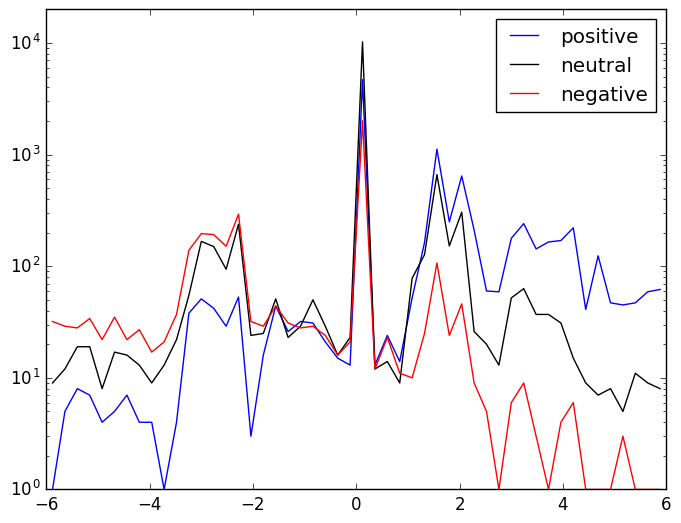
\includegraphics[width=\textwidth]{./figs/distrib/1500}
        \caption{Histogram for PMI lexicon, size 1\thinspace500}
        \label{fig:distrib_1500}
    \end{subfigure}
    \begin{subfigure}[b]{0.49\textwidth}
        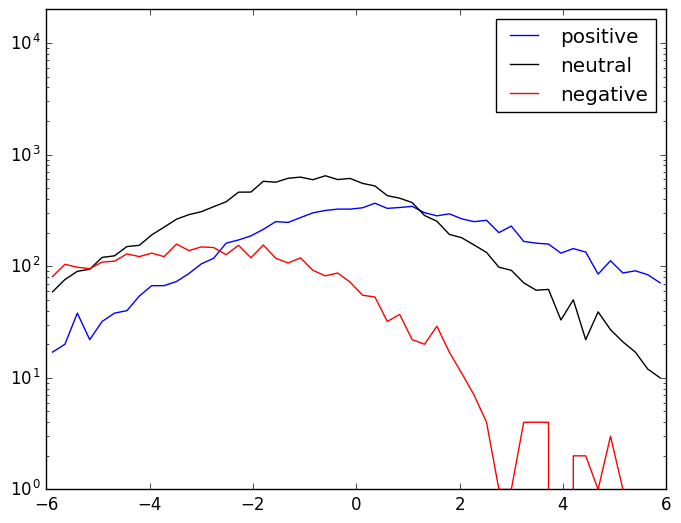
\includegraphics[width=\textwidth]{./figs/distrib/200000}
        \caption{Histogram for PMI lexicon, size 200\thinspace000}
        \label{fig:distrib_200000}
    \end{subfigure}
    \caption{Sentiment value histogram of small vs. large PMI Lexicon}
    \label{fig:distrib_size_comparison}
\end{figure}

Figure~\ref{fig:distrib_size_comparison} shows the distribution of positive, negative and neutral tweets given their sentiment value predicted by our classifier on a PMI lexicon of size 1\thinspace500 and of size 200\thinspace000. In comparison to Figure~\ref{fig:distrib_pmi}, showing the same distribution for our best PMI lexicon, the difference in performance is even further visualized. Compared to the distribution of our best PMI lexicon, the distribution of the 200\thinspace000 lexicon, shown in Figure~\ref{fig:distrib_200000} is almost an uniform distribution, the large spike around 0 is gone, but the differences between classes are smaller. The other extreme is the distribution of the small lexicon, shown in Figure~\ref{fig:distrib_1500}. It classifies some of the positive and negative tweets well, but most tweets are left with a score of 0.

\section{Best Performing PMI Lexicon}
After identifying our best performing PMI lexicon, a few statistics were gather in order to see whether or not the resulting lexicon contained the features we expected. It also provides a general insight into the lexicon created. \\

\begin{table}[t]
    \begin{tabular}{| l | l || l | l |}
        \hline
        \multicolumn{2}{|c||}{\textbf{Positive}} & \multicolumn{2}{c|}{\textbf{Negative}} \\ \hline
        \textbf{$n$-gram} & \textbf{Value} & \textbf{$n$-gram} & \textbf{Value} \\ \hline
        you have a great day        & 5.00 & a bad bitch        & -5.00 \\ \hline
        you have an amazing day     & 4.48 & bitch ass nigga    & -4.95 \\ \hline
        hope its a good one         & 4.33 & dumb ass           & -4.82 \\ \hline
        happy birthday i hope       & 4.21 & fuck that bitch    & -4.75 \\ \hline
        you had a great day         & 4.10 & fuck a bitch       & -4.75 \\ \hline
        you have a good day         & 4.08 & bad right now      & -4.73 \\ \hline
        you have a wonderful day    & 4.02 & weak ass           & -4.72 \\ \hline
        hope you have a great       & 4.01 & fuck this shit     & -4.68 \\ \hline
        you have a good one         & 3.99 & fuck fuck fuck     & -4.66 \\ \hline
        i love love love            & 3.96 & fool me twice      & -4.63 \\ \hline
    \end{tabular}
    \caption[Top 10 positive and negative entries in our lexicon]{The top 10 positive and negative entries in our best performing lexicon}
    \label{tab:lexicon_ngram_entries}
\end{table}

From Table~\ref{tab:lexicon_ngram_entries}, where the top 10 positive and negative lexicon entries are listed, we can clearly identify all of the top 10 positive as actual positive phrases and the top 10 negative as negative phrases. In addition we do not see any unigrams, meaning that our attempt of scoring longer $n$-grams higher/lower than shorter $n$-grams seems to be working.  \\

\begin{table}[t]
    \begin{tabular}{| c | l | l || c | l | l |}
        \hline
        \multicolumn{3}{|c||}{\textbf{Positive}} & \multicolumn{3}{c|}{\textbf{Negative}} \\ \hline
        \textbf{Emoji} & \textbf{Alias} & \textbf{Value} & \textbf{Emoji} & \textbf{Alias} & \textbf{Value} \\ \hline
        
\includegraphics[height=.5cm]{./figs/emojis/birthday} & Birthday Cake & 2.76 
        & 
\includegraphics[height=.5cm]{./figs/emojis/rage} & Pouting Face & -2.64 \\ \hline
        
\includegraphics[height=.5cm]{./figs/emojis/gift} & Wrapped Present & 2.60 
        & 
\includegraphics[height=.5cm]{./figs/emojis/parking} & Parking Sign & -2.41 \\ \hline
        
\includegraphics[height=.5cm]{./figs/emojis/balloon} & Balloon & 2.51 
        & 
\includegraphics[height=.5cm]{./figs/emojis/angry} & Angry Face & -2.41 \\ \hline
        
\includegraphics[height=.5cm]{./figs/emojis/confetti_ball} & Confetti Ball & 2.47 
        & 
\includegraphics[height=.5cm]{./figs/emojis/triumph} & Triumph Face & -2.40 \\ \hline
        
\includegraphics[height=.5cm]{./figs/emojis/party_popper} & Party Popper & 2.46 
        & 
\includegraphics[height=.5cm]{./figs/emojis/put_litter_in_its_place} & Litterbox & -2.34 \\ \hline
    \end{tabular}
    \caption[Top 5 positive and negative emojis in our lexicon]{The top 5 positive and negative emojis in our best performing lexicon}
    \label{tab:lexicon_emoji_entries}
\end{table}

Just like positive and negative phrases were separated with opposite sentiment values, the detected emojis were treated the same way, as seen in Table~\ref{tab:lexicon_emoji_entries}. All emojis listed as positive are commonly used to further express positive sentiment in positive sentences, while all of the emojis listed as negative are commonly used in negative sentences. \\

\begin{table}[t]
    \centering
    \begin{tabular}{| l | c |}
    \hline
    \textbf{$n$-gram} & \textbf{Value} \\ \hline
    you have a great day & 5.00  \\ \hline
    have a great day &  3.54 \\ \hline
    a great day & 2.16 \\ \hline
    great & 2.04 \\ \hline
    \end{tabular}
    \caption[Effect of $n$-gram length on sentiment value in our lexicon]{The effect of $n$-gram length on sentiment value}
    \label{tab:lexicon_entry_length_effect}
\end{table}

As mentioned earlier in this section, we wanted to create a lexicon where a long $n$-gram containing a polarized word should get a higher absolute sentiment value than a shorter $n$-gram containing the same word. In Table~\ref{tab:lexicon_entry_length_effect} this feature is identified through the four listed phrases containing the polarized word "great".

\section{Labeled Dataset Size Comparison}
\label{sec:labeled_dataset_size_comparison}
To better understand the relationship between the size of the labeled dataset and the performance of the resulting lexicon, we performed an experiment where we created lexica using different sized subsets of our \textit{Labeled} dataset. \\

\begin{table}[t]
    \centering
    \begin{tabular}{|r|c|c|c|c|}
        \hline
        \textbf{Labeled Size} & \textbf{2013} & \textbf{2014} & \textbf{2015} & \textbf{2016} \\ \hline
            50\thinspace000                 & 0.6002 & 0.5897 & 0.5584 & 0.5635 \\ \hline
            100\thinspace000                & 0.6262 & 0.6136 & 0.5830 & 0.5722 \\ \hline
            500\thinspace000                & 0.6601 & 0.6447 & 0.6142 & 0.5984 \\ \hline
            1\thinspace000\thinspace000     & 0.6686 & 0.6541 & 0.6130 & 0.6046 \\ \hline
            3\thinspace000\thinspace000     & 0.6677 & 0.6512 & 0.6153 & 0.6052 \\ \hline
            \bf 6\thinspace250\thinspace000 & 0.6748 & 0.6578 & 0.6201 & 0.6032 \\ \hline
    \end{tabular}
    \caption[Comparison of different sized labeled dataset]{Comparison of different sized labeled dataset after being tested on the 2013-2016 SemEval datasets.}
    \label{tab:labeled_size_comparison}   
\end{table}

Table~\ref{tab:labeled_size_comparison} shows the result of the experiment. The size of the labeled dataset seems to matter a lot at the beginning, but it quickly reaches a state where additional tweets provide almost no new information. This could be an artifact of the labeled dataset set creation method, since it includes only tweets containing words found in the \textit{AFINN} lexicon.


\section{Ablation Study}
\label{sec:ablation_study_lexicon_classifier}
To detect the impact each feature of both our lexicon creator and classifier impose on the performance, an ablation study was conducted. This was done by removing each feature in turn to see how the removal affected the system performance. Since our system, a lexicon based classifier using a PMI lexicon, is affected both by features used in the classification process and by features used in the creation process, the ablation study involved removing features from both processes. \\


\begin{table}[t]
    \centering
    \begin{tabular}{|l|c|c|c|c|}
        \hline
        \textbf{Features} & \textbf{2013} & \textbf{2014} & \textbf{2015} & \textbf{2016} \\ \hline
        All                         & 0.6748 & 0.6578 & 0.6201 & 0.6032 \\ \hline
        All - Adjectives/Adverbs    & 0.6653 & 0.6525 & 0.6127 & 0.6032 \\ \hline
        All - Negation              & 0.6732 & 0.6561 & 0.6180 & 0.6030 \\ \hline
        All - Intensification       & 0.6733 & 0.6548 & 0.6193 & 0.6036 \\ \hline
        All - PMI $n$-grams         & 0.6714 & 0.6503 & 0.6161 & 0.6010 \\ \hline
    \end{tabular}
    \caption[Ablation study results for lexicon classifier]{Ablation study results. All - F means all features except for F. All values are $F_1$-scores. The datasets used are the 2013-2016 SemEval datasets.}
    \label{tab:ablation_study_lexicon_classifier}   
\end{table}

As we can see from Table~\ref{tab:ablation_study_lexicon_classifier}, the impact each feature imposes on the performance of our classifier is very subtle, with the single most important feature being the adjective and adverb addition which increases the F1-score on the 2013 dataset by $0.01$. This means that the performance of our classifier almost entirely relies on the quality of our PMI lexicon, with the additional features only contributing a small amount. The second most important feature is our PMI $n$-grams used in the lexicon creation process. When replacing the PMI $n$-grams with frequency $n$-grams, $n$-grams selected solely based on their frequency, the F1-score drops by $0.0075$ on the 2014 dataset. Although we do see an improvement when using PMI $n$-grams over frequency $n$-grams, the small impact it has surprised us. By looking at the resulting lexica using the two $n$-gram approaches, the lexicon created with PMI $n$-grams looks far more promising than the lexicon created with frequency $n$-grams. \\

The small impact of negation and intensification is also somewhat surprising. While our lexicon excludes any $n$-gram containing intensifiers, negators are allowed. This is to better deal with common phrases containing negation, for example \textit{"glad im not the only one"} is an actual phrase included in one of our lexica, and its sentiment value is positive. Therefore some of the common negated phrases are already included in the lexicon and simply turning off the negation detection inside the classifier will only have an effect on less common phrases. The small effect of intensifiers is due to their low frequency, less than 1\% of the tweets contained any intensifiers.

\glsresetall

